\chapter{Introduction to Deep Learning}

Artificial intelligence is the start to outsourcing brain function to man-made machines.  A machine is said to have ``Artificial Intelligence'' if it can do what people say requires intelligence \cite{jackson2019introduction}, from counting monetary denominations to surveying Mars, playing chess games to converting human speech.  Within the realm of this is the subcategory \textit{machine learning}, in which models are tested based on training data in order to ``teach'' them right from wrong.  Machine learning has an increased emphasis on the use of computers in statistical analyses and a decreased emphasis on proving confidence intervals around them \cite{Goodfellow-et-al-2016}.  With astronomical advances in modern computing technology, creating elaborate learning models with raised functionality has become more and more accessible, creating a new category known as \textit{deep learning}, which is the parent of the subjects within this thesis.  Deep learning models operate beyond those of traditional machine learning as such models contain layers of complexities, each performing a specific task for the overall objective.  Algorithms and procedures unite with complex mathematical formulas to generate extremely precise models without the assumptions of linear models.

%---EXAMPLE FOR PHOTOS--
%--- https://www.overleaf.com/learn/latex/Inserting_Images ---for reference
%\begin{figure}[h]
%    \centering
%    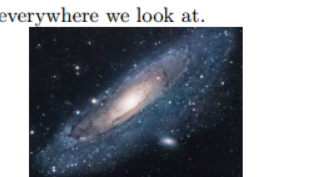
\includegraphics[width=0.25\textwidth]{poo}
%    \caption{a nice plot}
%    \label{fig:mesh1}
%\end{figure}


\section{Overview} %-------------SECTION

Anymore, the field of statistics is closely intertwined with computer science, if not married to it.  One cannot exist without the other and maintain the state of knowledge their union has to offer.  Deep learning is proof in and of itself of this.
Deep learning is the brand of machine learning concerned with using Artificial Neural Networks (ANN's) to reveal complex abstractions within data.
The evolution of the process of mimicking cognitive brain functionality within artificial machines dates back to the 1940's under the term \textit{cybernetics}, which was originally intended to provide computational models for biological understanding \cite{Goodfellow-et-al-2016}.  Since then, the history of what we now call ``deep learning'' has undergone waves of renaissance.  

\subsection{Working with Structured Data} %-------------SECTION

It is perhaps the responsibility of the statistician more than the computer scientist to perform certain measures when given structured data.  A data set determined by numbers, labels, predictor and response variables, timestamps and factors is what is meant by structured data.  It has a direct connection to mathematical theory.  With it, such analytical tasks can be performed as a regression, classification, missing value imputation, outlier detection, and more.


\subsection{Working with Unstructured Data} %-------------SECTION

In the case of unstructured data, the computer scientist may take role as the primary authority.  An image, sound wave, even human perception \cite{anbarasan2022human} can be delivered to a computer to sense.  Such data must be coerced into a numeric format in order to be analyzed: a sound wave into an image; an image into a matrix of pixel values.  A common elementary application to deep learning is to utilize a network to recognize and classify image date based on the pixel values, as is shown in Figure \ref{minecraft}.  In image data, each pixel is an input value determined by a number corresponding to that specific color.  For grayscale image data, that number is a value from 0 to 1.  Color images are represented as vectors of three values (RGB).

\begin{figure}[H]
    \centering
%\raisebox{20pt}
    
\includegraphics[width=.2\textwidth]{Figures/pickaxe_1.png}
    \hspace{60pt}
    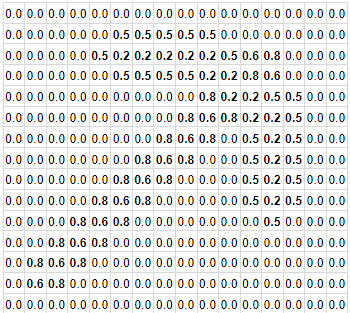
\includegraphics[width=.5\textwidth]{Figures/pickaxe_2.png}
    \caption{\footnotesize{An 16x16 pixel image, with its numerical counterpart next to it.  In greyscale image data, a value of 0.0 corresponds to white, 1.0 to black, and ordered variations of gray to values in between}}
    \label{minecraft}
\end{figure}

\begin{comment}
Any type of data can be modeled with a deep learning neural network, provided there is enough of it to match the complexity if the model.  Image data tends to have a great number of inputs to begin with.  In the world of big data, finding material to work with is no trouble.  
\end{comment}

Structured or not, large data or small, regression or classification, through frequentism or Bayes; there is a neural network for that.
Neural networks are often described as black boxes; given an input, the blur of functionality within hidden layers returns an output.  This thesis is presented to reveal some of the complexities of these high-level machines.  It begins with a review of the basic structure of the Multi-Layer Perception, and describes variants associated with a change of architecture.  It continues with research on Bayesian methods, based both in theory and inclusive of practical estimation techniques to apply Bayes.  It closes out with a return to deep learning discussion and how Bayes can be applied to these intricate models.